\newpage \subsection{Μελέτη επίδρασης παραμέτρων ιεραρχίας μνήμης στην απόδοση της εφαρμογής για μεταβλητό κύκλο ρολογιού}
\vspace{3mm}


Στο κομμάτι αυτό της εργασίας γίνεται σχολιασμός των αποτελεσμάτων των
προηγούμενων πειραμάτων, θεωρώντας όμως ότι ο κύκλος του ρολογιού μεταβάλλεται
καθώς αλλάζουν τα χαρακτηριστικά των L1 Cache, L2 Cache, TLB. Σχολιάζουμε την
επίδοση των διαφορετικών benchmarks θεωρώντας κάθε φορά ως αρχικό σημείο
αναφοράς τη πρώτη προσομοίωση για το καθένα από αυτά και πως διπλασιασμός του
associativity ή του μεγέθους (size) προκαλεί αύξηση του κύκλου κατά 5 \% ή 10\%
αντίστοιχα. 

\textbf{Συγκεκριμένα, θεωρώντας ως αρχικό κύκλο αναφοράς τον κύκλος της
πρώτης προσομοίωσης, σχεδιάζουμε διαγράμματα στα οποία \color{red} το ipc αντιπροσωπεύει το
πλήθος των εντολών που εκτελούνται σε χρνικό διάστημα ίσο με τον αρχικό κύκλο
αναφοράς.}


%----------------L1 Cache-----------------------
\subsubsection{L1 Cache}
\begin{minipage}{\textwidth}
    \begin{center}
        \fbox{\textlatin{\textbf{\textit{blackscholes}}}}\\
        \vspace{3mm}
        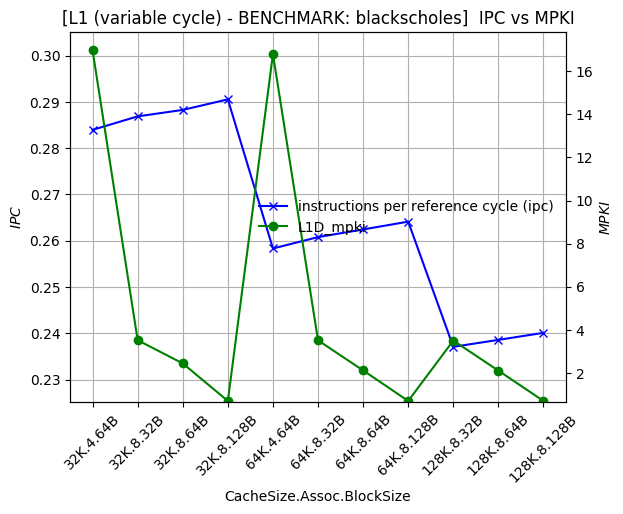
\includegraphics[scale=0.65]{graphs/L1/var/blackscholes.png}
        \vspace{6mm}
    \end{center}
\end{minipage}


\begin{minipage}{\textwidth}
    \begin{center}
        \fbox{\textlatin{\textbf{\textit{bodytrack}}}}\\
        \vspace{3mm}
        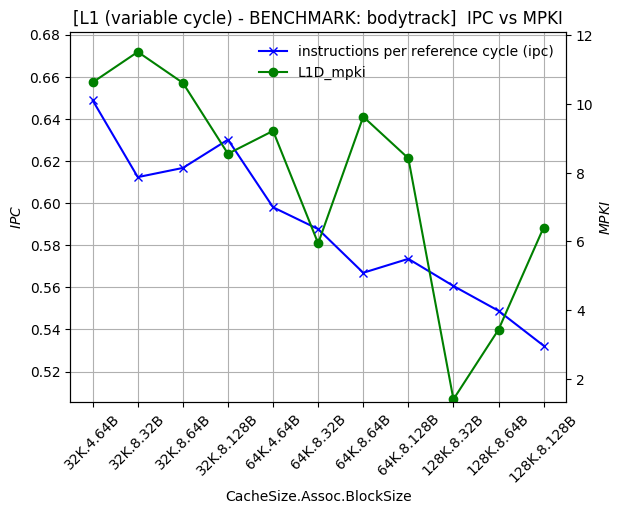
\includegraphics[scale=0.65]{graphs/L1/var/bodytrack.png}
        \vspace{6mm}
    \end{center}
\end{minipage}

\begin{minipage}{\textwidth}
    \begin{center}
        \fbox{\textlatin{\textbf{\textit{canneal}}}}\\
        \vspace{3mm}
        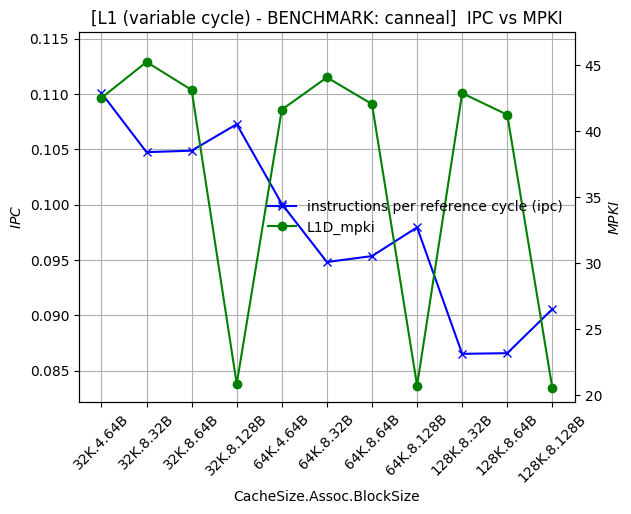
\includegraphics[scale=0.65]{graphs/L1/var/canneal.png}
        \vspace{6mm}
    \end{center}
\end{minipage}

\begin{minipage}{\textwidth}
    \begin{center}
        \fbox{\textlatin{\textbf{\textit{facesim}}}}\\
        \vspace{3mm}
        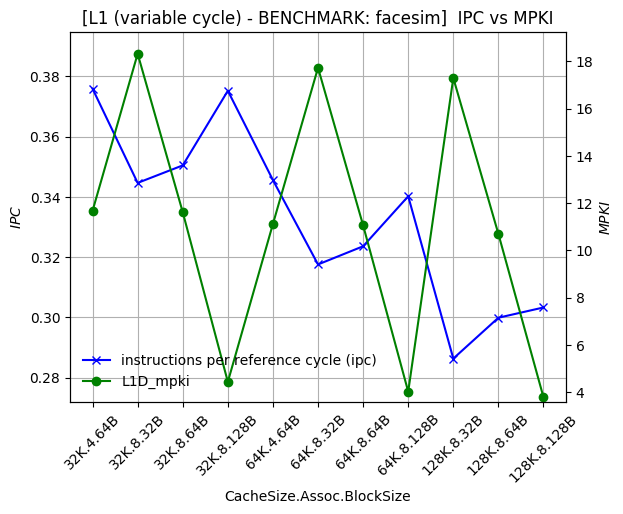
\includegraphics[scale=0.65]{graphs/L1/var/facesim.png}
        \vspace{6mm}
    \end{center}
\end{minipage}

\begin{minipage}{\textwidth}
    \begin{center}
        \fbox{\textlatin{\textbf{\textit{ferret}}}}\\
        \vspace{3mm}
        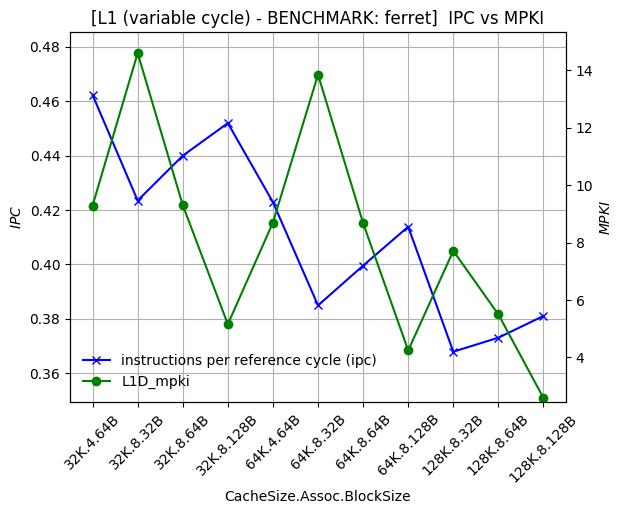
\includegraphics[scale=0.65]{graphs/L1/var/ferret.png}
        \vspace{6mm}
    \end{center}
\end{minipage}


\begin{minipage}{\textwidth}
    \begin{center}
        \fbox{\textlatin{\textbf{\textit{fluidanimate}}}}\\
        \vspace{3mm}
        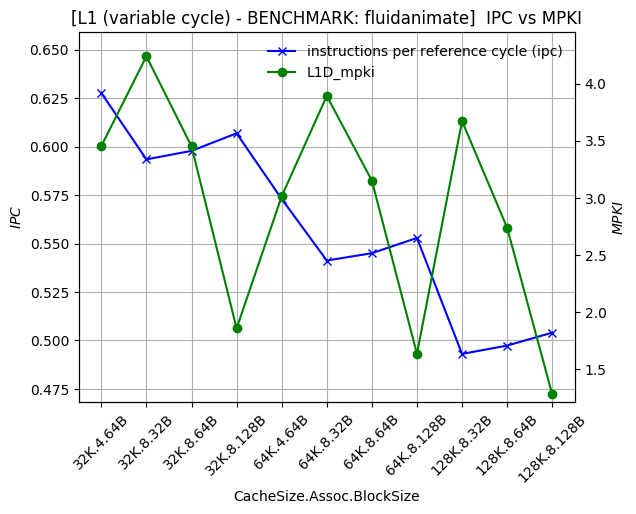
\includegraphics[scale=0.65]{graphs/L1/var/fluidanimate.png}
        \vspace{6mm}
    \end{center}
\end{minipage}

\begin{minipage}{\textwidth}
    \begin{center}
        \fbox{\textlatin{\textbf{\textit{freqmine}}}}\\
        \vspace{3mm}
        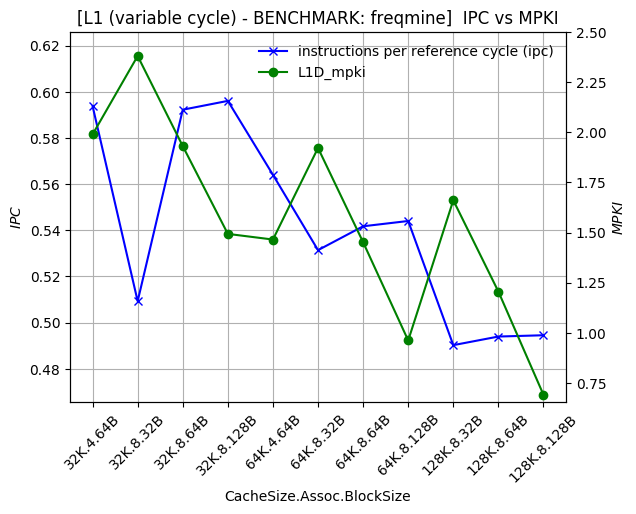
\includegraphics[scale=0.65]{graphs/L1/var/freqmine.png}
        \vspace{6mm}
    \end{center}
\end{minipage}

\begin{minipage}{\textwidth}
    \begin{center}
        \fbox{\textlatin{\textbf{\textit{rtview}}}}\\
        \vspace{3mm}
        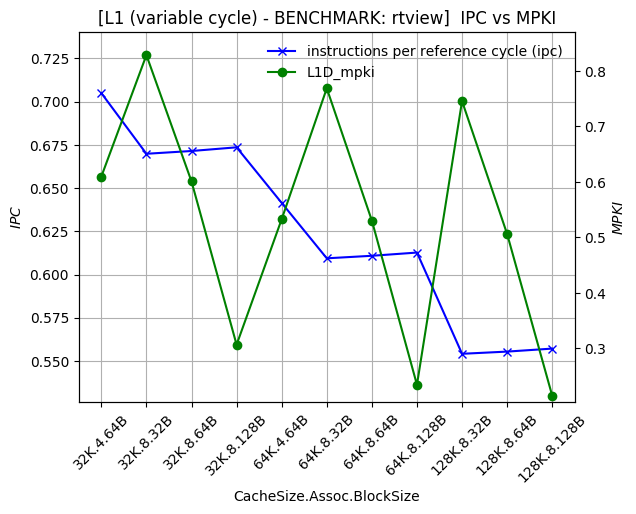
\includegraphics[scale=0.65]{graphs/L1/var/rtview.png}
        \vspace{6mm}
    \end{center}
\end{minipage}

\begin{minipage}{\textwidth}
    \begin{center}
        \fbox{\textlatin{\textbf{\textit{streamcluster}}}}\\
        \vspace{3mm}
        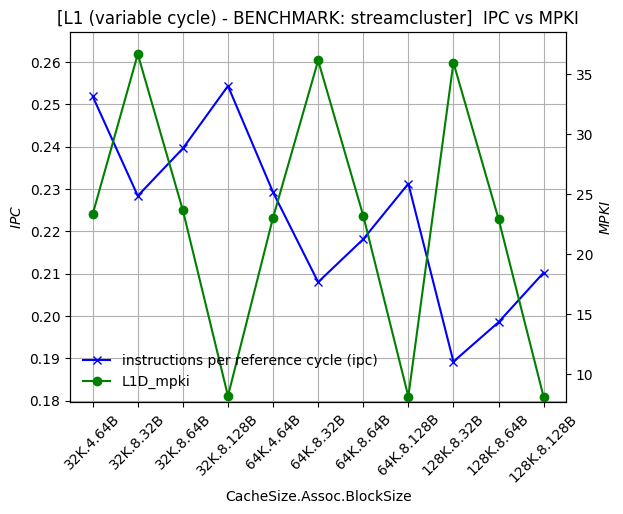
\includegraphics[scale=0.65]{graphs/L1/var/streamcluster.png}
        \vspace{6mm}
    \end{center}
\end{minipage}

\begin{minipage}{\textwidth}
    \begin{center}
        \fbox{\textlatin{\textbf{\textit{swaptions}}}}\\
        \vspace{3mm}
        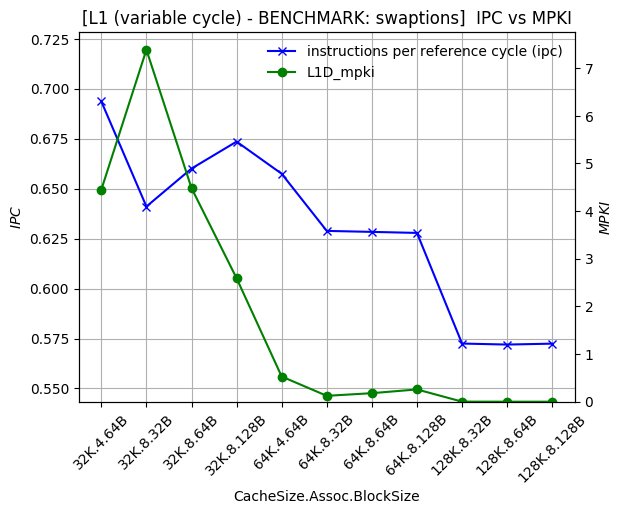
\includegraphics[scale=0.65]{graphs/L1/var/swaptions.png}
        \vspace{6mm}
    \end{center}
\end{minipage}

\begin{minipage}{\textwidth}
    \begin{center}
        \fbox{\textlatin{\textbf{\textit{Geometric Average}}}}\\
        \vspace{3mm}
        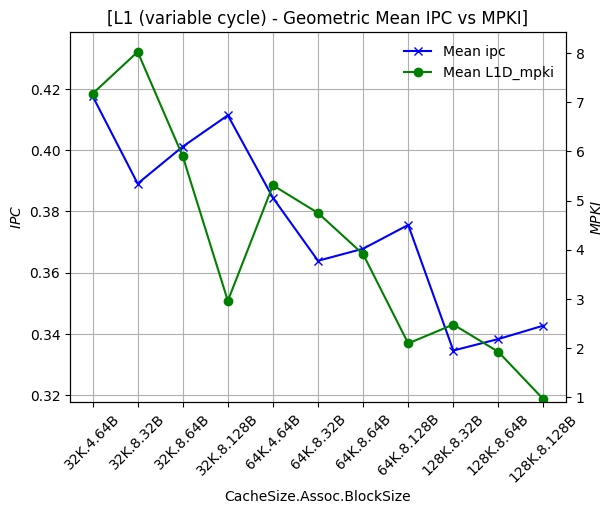
\includegraphics[scale=0.60]{graphs/L1/var/mean.png}
        \vspace{6mm}
    \end{center}
\end{minipage}

\newpage
\begin{center}
    \textbf{Συμπεράσματα για την \textlatin{L1 Cache}}    
\end{center}

Παρατηρούμε πως πλέον δεν είναι απαραίτητα αντιστρόφως ανάλογα τα μεγέθη
\textlatin{IPC, MPKI}. Καθώς, όπως αναφέραμε, πλέον το IPC αναφέρεται στον
αρχικό κύκλο του πειράματος αναφοράς, πλέον ενώ μπορεί να αυξάνονται οι εντολές
που εκτελούνται στον νέο κύκλο, η διάρκεια του κύκλου λόγω μεταβολής ενδέχεται
να είναι αρκετά μεγαλύτερη σε σχέση με τον κύκλο αναφοράς οπότε και η επίδοση,
δηλαδή οι εντολές ανα χρονικό διάστημα να μην είναι καλή.

Είναι εμφανές ότι η μεταβολή των χαρακτηριστικών της L1 Cache επιδρά ή αρνητικά 
ή χωρίς καμία μεταβολή στην επίδοση, καθώς οι εντολές που εκτελούνται στον αρχικό 
κύκλο αναφοράς ή μειώνονται ή παραμένουν σταθερές. Επομένως σε κάθε περίπτωση, 
η βέλιτση επιλογή είναι η 32K.4.64B L1 Cache.


%\newpage ----------------L2 Cache-----------------------
\newpage
\subsubsection{L2 Cache}

\begin{minipage}{\textwidth}
    \begin{center}
        \fbox{\textlatin{\textbf{\textit{blackscholes}}}}\\
        \vspace{3mm}
        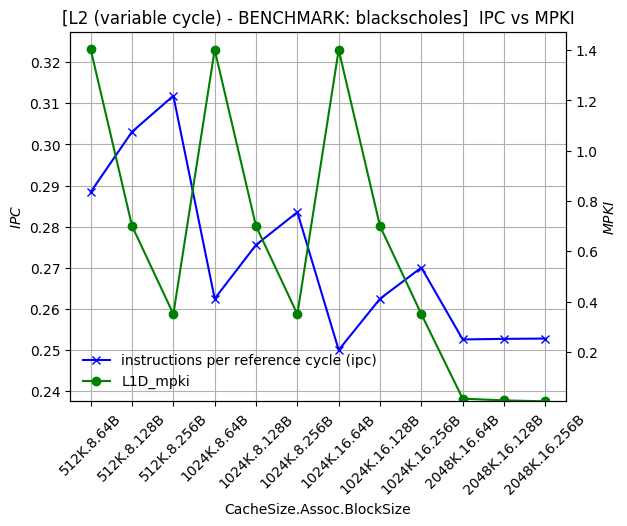
\includegraphics[scale=0.65]{graphs/L2/var/blackscholes.png}
        \vspace{6mm}
    \end{center}
\end{minipage}


\begin{minipage}{\textwidth}
    \begin{center}
        \fbox{\textlatin{\textbf{\textit{bodytrack}}}}\\
        \vspace{3mm}
        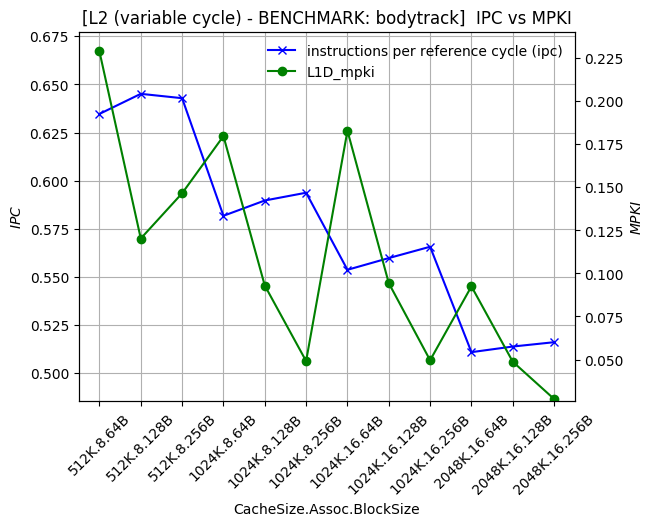
\includegraphics[scale=0.65]{graphs/L2/var/bodytrack.png}
        \vspace{6mm}
    \end{center}
\end{minipage}

\begin{minipage}{\textwidth}
    \begin{center}
        \fbox{\textlatin{\textbf{\textit{canneal}}}}\\
        \vspace{3mm}
        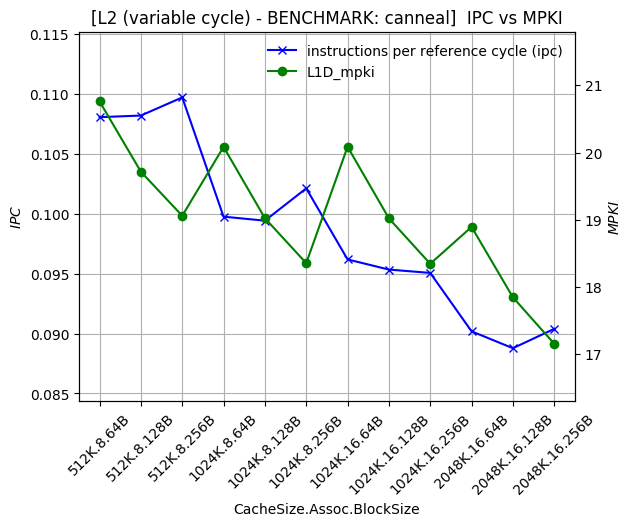
\includegraphics[scale=0.65]{graphs/L2/var/canneal.png}
        \vspace{6mm}
    \end{center}
\end{minipage}

\begin{minipage}{\textwidth}
    \begin{center}
        \fbox{\textlatin{\textbf{\textit{facesim}}}}\\
        \vspace{3mm}
        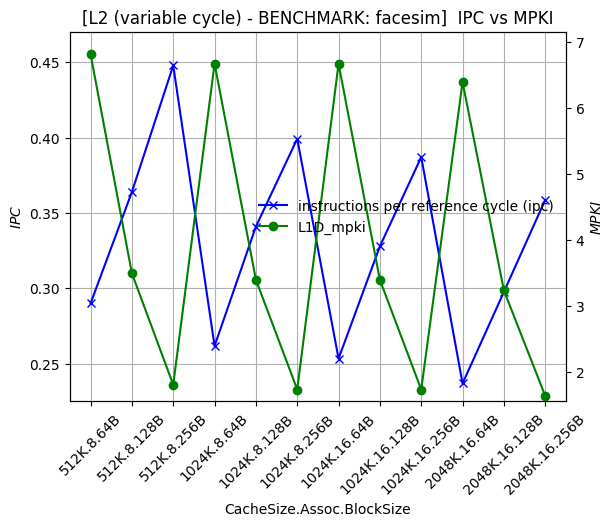
\includegraphics[scale=0.65]{graphs/L2/var/facesim.png}
        \vspace{6mm}
    \end{center}
\end{minipage}

\begin{minipage}{\textwidth}
    \begin{center}
        \fbox{\textlatin{\textbf{\textit{ferret}}}}\\
        \vspace{3mm}
        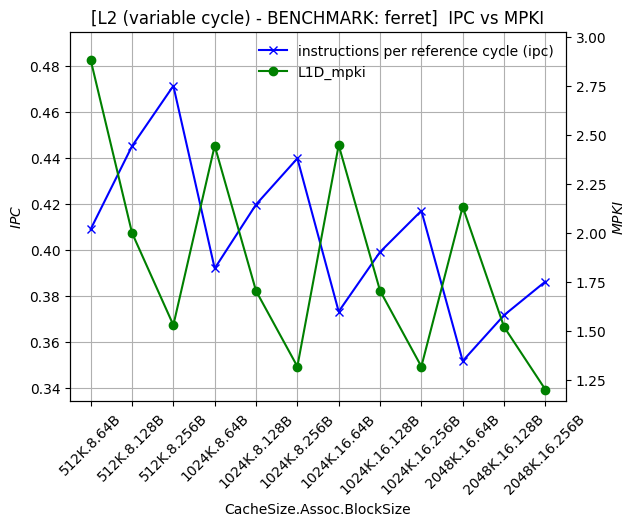
\includegraphics[scale=0.65]{graphs/L2/var/ferret.png}
        \vspace{6mm}
    \end{center}
\end{minipage}


\begin{minipage}{\textwidth}
    \begin{center}
        \fbox{\textlatin{\textbf{\textit{fluidanimate}}}}\\
        \vspace{3mm}
        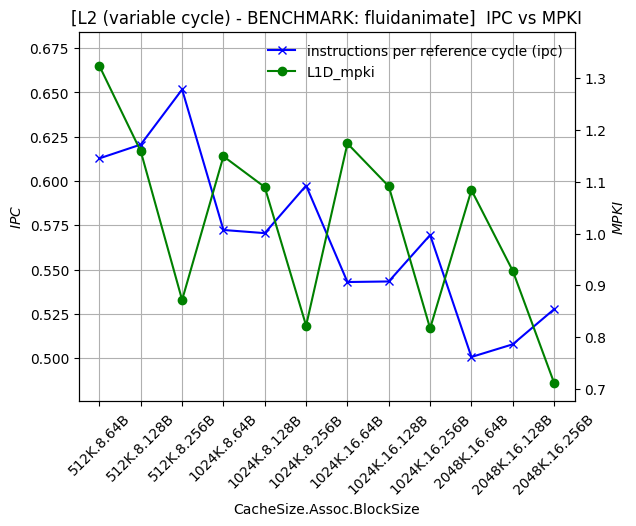
\includegraphics[scale=0.65]{graphs/L2/var/fluidanimate.png}
        \vspace{6mm}
    \end{center}
\end{minipage}

\begin{minipage}{\textwidth}
    \begin{center}
        \fbox{\textlatin{\textbf{\textit{freqmine}}}}\\
        \vspace{3mm}
        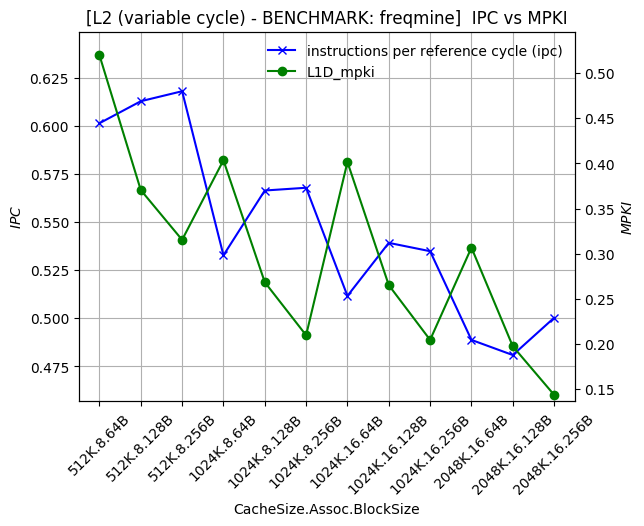
\includegraphics[scale=0.65]{graphs/L2/var/freqmine.png}
        \vspace{6mm}
    \end{center}
\end{minipage}

\begin{minipage}{\textwidth}
    \begin{center}
        \fbox{\textlatin{\textbf{\textit{rtview}}}}\\
        \vspace{3mm}
        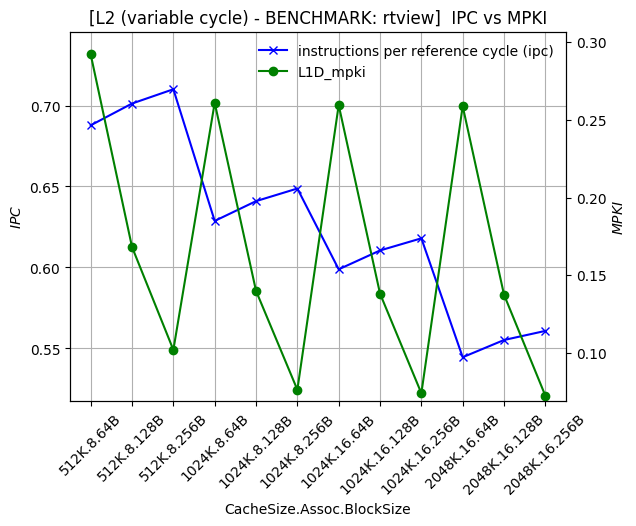
\includegraphics[scale=0.65]{graphs/L2/var/rtview.png}
        \vspace{6mm}
    \end{center}
\end{minipage}

\begin{minipage}{\textwidth}
    \begin{center}
        \fbox{\textlatin{\textbf{\textit{streamcluster}}}}\\
        \vspace{3mm}
        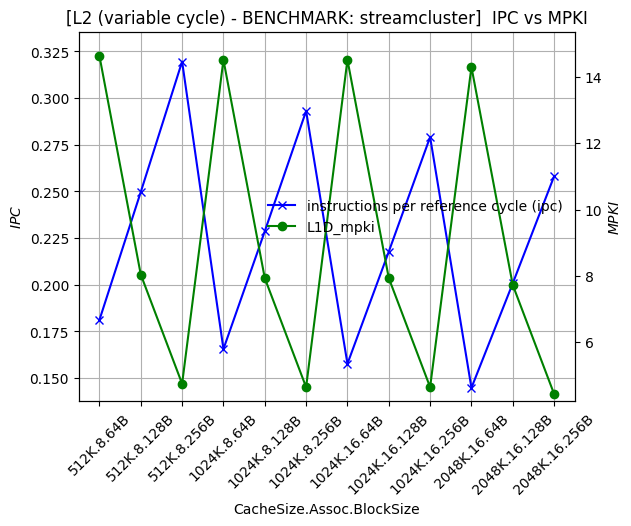
\includegraphics[scale=0.65]{graphs/L2/var/streamcluster.png}
        \vspace{6mm}
    \end{center}
\end{minipage}

\begin{minipage}{\textwidth}
    \begin{center}
        \fbox{\textlatin{\textbf{\textit{swaptions}}}}\\
        \vspace{3mm}
        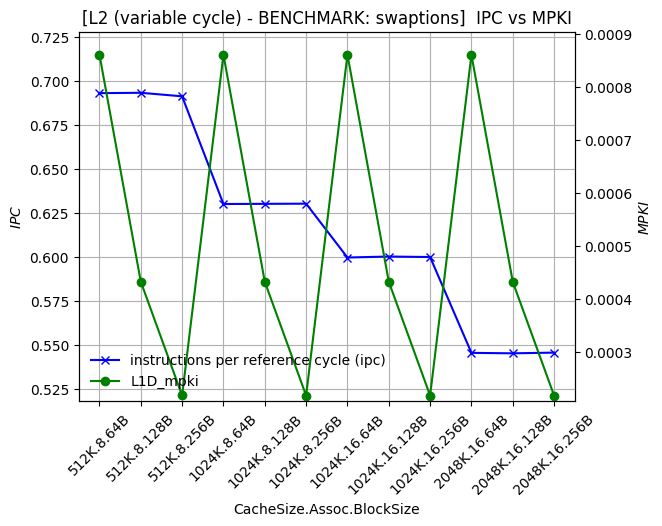
\includegraphics[scale=0.65]{graphs/L2/var/swaptions.png}
        \vspace{6mm}
    \end{center}
\end{minipage}

\begin{minipage}{\textwidth}
    \begin{center}
        \fbox{\textlatin{\textbf{\textit{Geometric Average}}}}\\
        \vspace{3mm}
        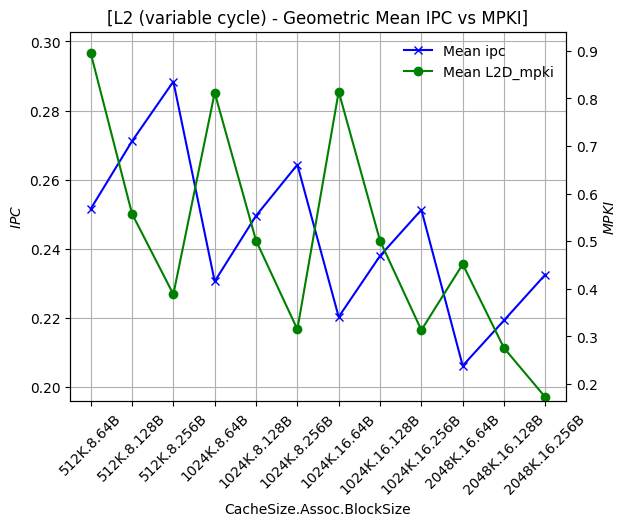
\includegraphics[scale=0.60]{graphs/L2/var/mean.png}
        \vspace{6mm}
    \end{center}
\end{minipage}

\begin{center}
    \textbf{Συμπεράσματα για την \textlatin{L2 Cache}}    
\end{center}



Όπως και για την L1, έτσι και για την L2 δεν είναι απαραίτητα αντιστρόφως
ανάλογα τα μεγέθη \textlatin{IPC, MPKI}. Καθώς, όπως αναφέραμε, πλέον το IPC
αναφέρεται στον αρχικό κύκλο του πειράματος αναφοράς, πλέον ενώ μπορεί μεν να
αυξάνονται οι εντολές που εκτελούνται στον νέο κύκλο, η διάρκεια του κύκλου λόγω
μεταβολής ενδέχεται να είναι αρκετά μεγαλύτερη σε σχέση με τον κύκλο αναφοράς
οπότε και η επίδοση, δηλαδή οι εντολές ανα χρονικό διάστημα να μην είναι καλή.

\begin{enumerate}
    \item Σε όλα τα bencmarks βλέπουμε πως η επίδοση μειώνεται καθώς αυξάνεται
        το associativity ή το μέγεθος της L2. Αυτό συμβαίνει καθώς ο κύκλος του
        ρολογιού αυξάνεται πιο γρήγορα σε σχέση με το πόσες περισσότερες εντολές
        εκτελούνται στον νέο κύκλο.
    \item  Για σταθερά τα υπόλοιπα χαρακτηριστικά, η αύξηση του block size
    επιφέρει σε όλα τα benchmarks σημαντική βελτίωση της επίδοσης (εκτός από το benchmark
    swaptions που δεν επηρεάζεται). 
\end{enumerate}

\textit{Από τα επιμέρους διαγράμαμτα του κάθε benchmark αλλά και από τον γεωμετρικό τους μέσο, είναι προφανές πως
ο 3ος συνδυασμός, 512Κ.8.256Β αποτελεί τη βέλτιστη δυνατή επιλογή για την \textlatin{L2 Cache}.}
\vspace{1cm}

\newpage
%----------------TLB-----------------------
\subsubsection{TLB}

\begin{minipage}{\textwidth}
    \begin{center}
        \fbox{\textlatin{\textbf{\textit{blackscholes}}}}\\
        \vspace{3mm}
        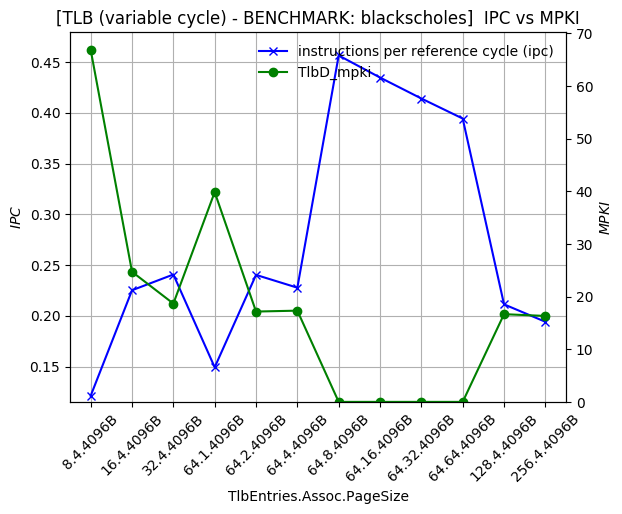
\includegraphics[scale=0.65]{graphs/TLB/var/blackscholes.png}
        \vspace{6mm}
    \end{center}
\end{minipage}


\begin{minipage}{\textwidth}
    \begin{center}
        \fbox{\textlatin{\textbf{\textit{bodytrack}}}}\\
        \vspace{3mm}
        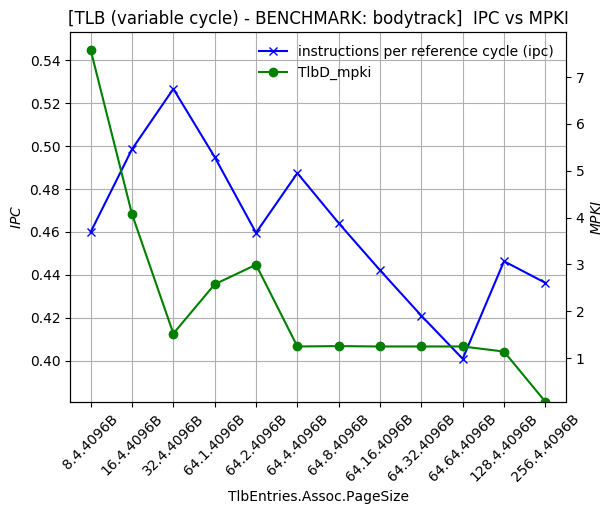
\includegraphics[scale=0.65]{graphs/TLB/var/bodytrack.png}
        \vspace{6mm}
    \end{center}
\end{minipage}

\begin{minipage}{\textwidth}
    \begin{center}
        \fbox{\textlatin{\textbf{\textit{canneal}}}}\\
        \vspace{3mm}
        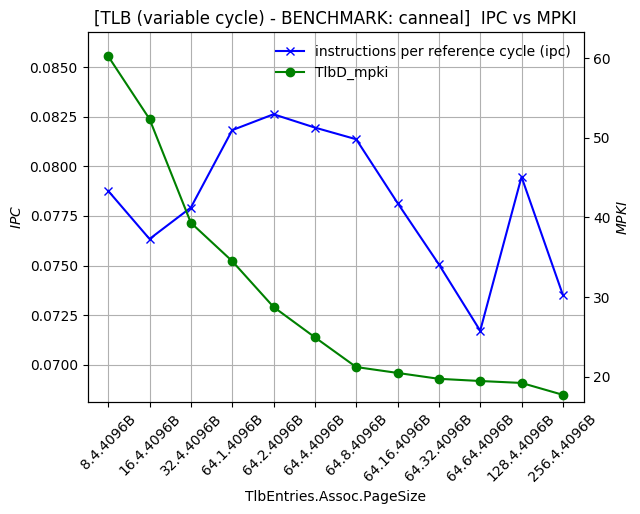
\includegraphics[scale=0.65]{graphs/TLB/var/canneal.png}
        \vspace{6mm}
    \end{center}
\end{minipage}

\begin{minipage}{\textwidth}
    \begin{center}
        \fbox{\textlatin{\textbf{\textit{facesim}}}}\\
        \vspace{3mm}
        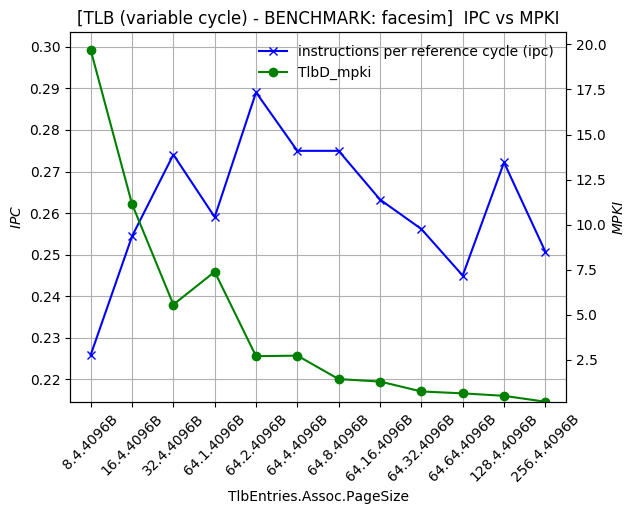
\includegraphics[scale=0.65]{graphs/TLB/var/facesim.png}
        \vspace{6mm}
    \end{center}
\end{minipage}

\begin{minipage}{\textwidth}
    \begin{center}
        \fbox{\textlatin{\textbf{\textit{ferret}}}}\\
        \vspace{3mm}
        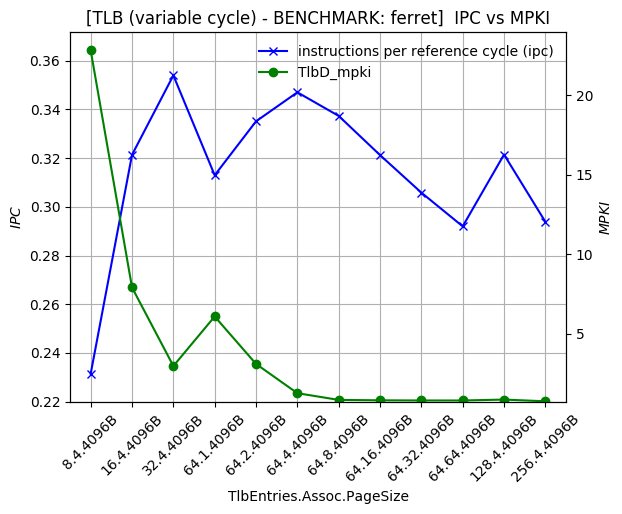
\includegraphics[scale=0.65]{graphs/TLB/var/ferret.png}
        \vspace{6mm}
    \end{center}
\end{minipage}


\begin{minipage}{\textwidth}
    \begin{center}
        \fbox{\textlatin{\textbf{\textit{fluidanimate}}}}\\
        \vspace{3mm}
        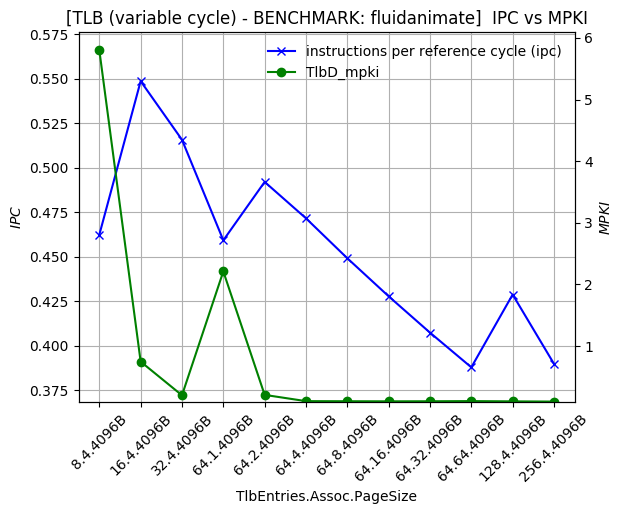
\includegraphics[scale=0.65]{graphs/TLB/var/fluidanimate.png}
        \vspace{6mm}
    \end{center}
\end{minipage}

\begin{minipage}{\textwidth}
    \begin{center}
        \fbox{\textlatin{\textbf{\textit{freqmine}}}}\\
        \vspace{3mm}
        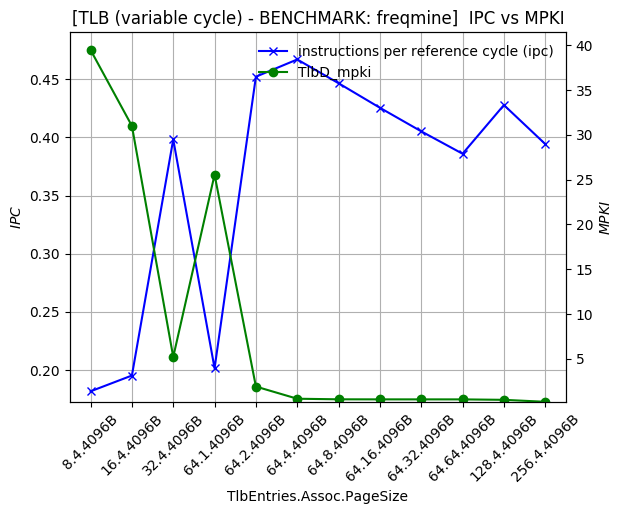
\includegraphics[scale=0.65]{graphs/TLB/var/freqmine.png}
        \vspace{6mm}
    \end{center}
\end{minipage}

\begin{minipage}{\textwidth}
    \begin{center}
        \fbox{\textlatin{\textbf{\textit{rtview}}}}\\
        \vspace{3mm}
        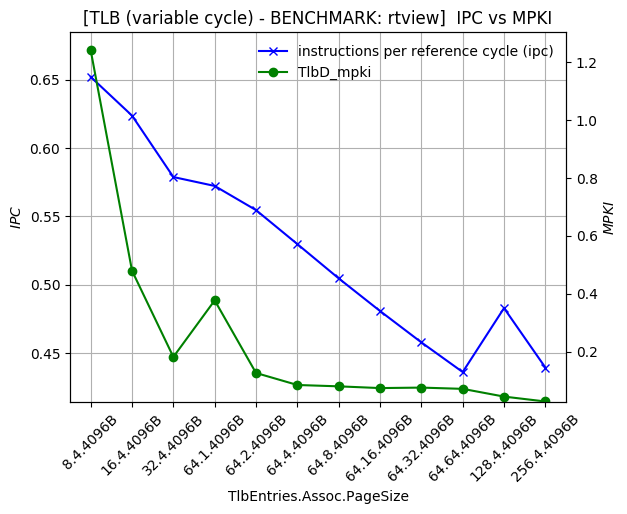
\includegraphics[scale=0.65]{graphs/TLB/var/rtview.png}
        \vspace{6mm}
    \end{center}
\end{minipage}

\begin{minipage}{\textwidth}
    \begin{center}
        \fbox{\textlatin{\textbf{\textit{streamcluster}}}}\\
        \vspace{3mm}
        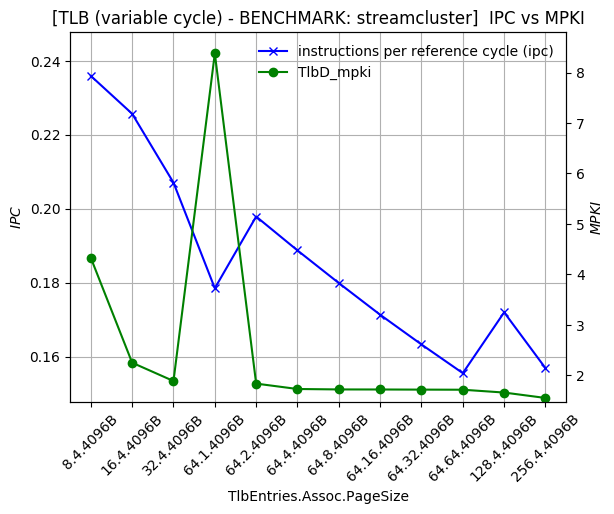
\includegraphics[scale=0.65]{graphs/TLB/var/streamcluster.png}
        \vspace{6mm}
    \end{center}
\end{minipage}

\begin{minipage}{\textwidth}
    \begin{center}
        \fbox{\textlatin{\textbf{\textit{swaptions}}}}\\
        \vspace{3mm}
        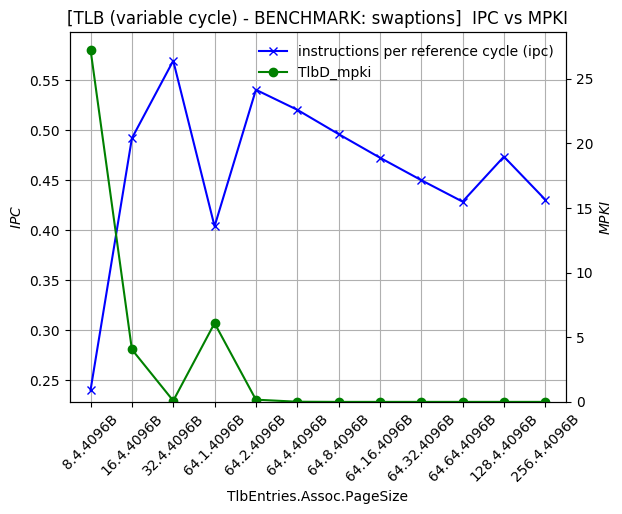
\includegraphics[scale=0.65]{graphs/TLB/var/swaptions.png}
        \vspace{6mm}
    \end{center}
\end{minipage}

\begin{minipage}{\textwidth}
    \begin{center}
        \fbox{\textlatin{\textbf{\textit{Geometric Average}}}}\\
        \vspace{3mm}
        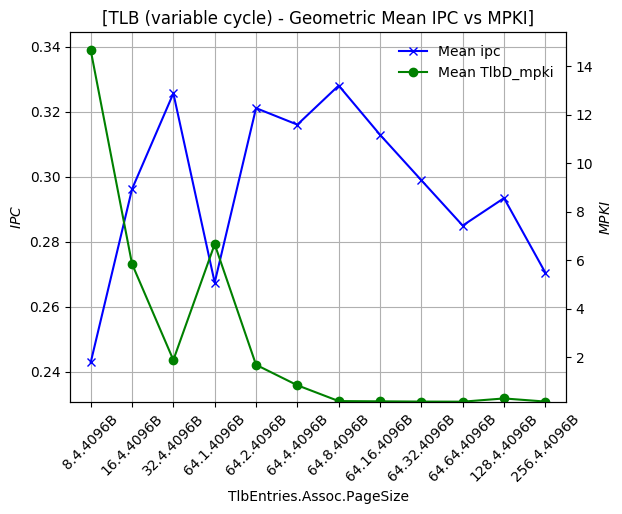
\includegraphics[scale=0.60]{graphs/TLB/var/mean.png}
        \vspace{6mm}
    \end{center}
\end{minipage}


\begin{center}
    \textbf{Συμπεράσματα για το \textlatin{TLB}}    
\end{center}

Σε γενικές γραμμές, παρατηρούμε να μεταβάλλονται αντιστρόφως ανάλογα τα μεγέθη
\textlatin{IPC, MPKI}. Αυτό είναι λογικό αφού όσο περισσότερες αστοχίες
γίνονται, τόσο χειρότερη επίδοση θα έχουμε (άρα και μικρότερο \textlatin{IPC})
και αντίστροφα. 
\begin{enumerate}
    \item Σε όλα τα παραπάνω bencmarks, για μέγεθος TLB 64 η αλλαγή του
    associativity από 1 σε 2 ή και 4 οδηγεί σε βελτίωση της επίδοσης κατά μέσο
    όρο. Από το σημείο αυτό και πέρα ωστόσο, για μέγεθος 64 κάθε διπλασιασμός
    του associativity οδηγεί σε μείωση της επίδοσης με γραμμικό τρόπο.

    \item Στο swaptions η καλύτερη επίδοση επιτυγχάνεται για 32.4.4096B. Συγκεκριμένα
    για σταθερό το associativity = 4 και το Page Size, η αυξηση των TLB Entries
    από 8 μέχρι 32 οδηγεί σε βελτίωση της επίδοσης, ενώ από 32 σε 64 μειώνει την
    επίδοση.
   
    \item Στα benchmark swaptions και rtview η καλύτερη επίδοση επιτυγχάνεται για το
    αρχικό configuration 8.4.4096B.

\end{enumerate}

\textit{Γενικότερα, κάθε bencmark επηρεάζεται με διαφορετικό τρόπο από τα χαρακτηριστικά
της TLB. Με βάσει τα διαγράμματα των γεωμετρικών μέσων ωστόσο, μπορούμε να πούμε
πως 2 σχετικά καλοί και προτιμητέοι συνδυασμοί είναι οι 32.4.4096, 64.2.4096 και
64.8.4096.}

\vspace{1cm}